\de{ĐỀ THI HỌC KỲ II NĂM HỌC 2022-2023}{THPT Củ Chi}

\begin{bt}%[0T7B1-1]%[Dự án đề kiểm tra HKII NH22-23-Võ Thị Thùy Trang]%[THPT CU CHI]
	\immini{ Dựa vào đồ thị của hàm số bậc hai ở hình bên, hãy lập và kết luận bảng xét dấu của tam thức bậc hai.}
{\begin{tikzpicture}[scale=.7,>=stealth, font=\footnotesize, line join=round, line cap=round]
		\def\a{1} \def\b{-4} \def\c{4} % Hệ số
		\def\xmin{-1} \def\xmax{5}
		\def\ymin{-1} \def\ymax{5}
%		\draw[color=gray!50,dashed] (\xmin,\ymin) grid (\xmax,\ymax);
		\draw[->] (\xmin,0)--(\xmax,0) node [below]{$x$};
		\draw[->] (0,\ymin)--(0,\ymax) node [left]{$y$};
		\node at (0,0) [below left]{$O$};
		\node at (2,0) [below]{$2$};
		\clip (\xmin+0.1,\ymin+0.1) rectangle (\xmax-0.5,\ymax-0.1);
		\draw[smooth,samples=300] plot(\x,{\a*(\x)^2+\b*(\x)+\c});
\end{tikzpicture}}
\loigiai{
	Bảng xét dấu
	\begin{center}
		
\begin{tikzpicture}
			\tkzTabInit[nocadre=true,lgt=2,espcl=2,deltacl=0.6]
			{$x$ /0.6,$f(x)$ /0.6}
			{$-\infty$,$2$,$+\infty$}
			\tkzTabLine{,+,$0$,+,}
		\end{tikzpicture}
	\end{center}
Do đó $f(x)\ge 0$, $\forall x\in \mathbb{R}$.
}
\end{bt}
\begin{bt}%[0T7B3-2]%[Dự án đề kiểm tra HKII NH22-23-Võ Thị Thùy Trang]%[THPT CU CHI]
	Giải phương trình $\sqrt{6 x^2-22 x+14}=\sqrt{4 x^2-11 x-1}$
	\loigiai{Ta có 
		\allowdisplaybreaks
		\begin{eqnarray*}
			&&\sqrt{6 x^2-22 x+14}=\sqrt{4 x^2-11 x-1}\\
			& \Rightarrow & 6 x^2-22 x+14=4 x^2-11 x-1\\
			& \Leftrightarrow & 2x^2-11x+15=0 \Leftrightarrow \hoac{&x=3\\&x=\dfrac{5}{2}.}
		\end{eqnarray*}
	Thử lại ta thấy chỉ có $x=3$ thỏa phương trình nên phương trình đã cho có một nghiệm là $x=3$.
	}
\end{bt}
\begin{bt}%[0T8B2-1]%[Dự án đề kiểm tra HKII NH22-23-Võ Thị Thùy Trang]%[THPT CU CHI]
	\begin{enumerate}
		\item Có bao nhiêu cách chia $12$ người thành ba nhóm lần lượt có $5$ người, $4$ người, $3$ người.
		\item Có bao nhiêu cách xếp $5$ bạn Nhân, Lễ, Nghĩa, Trí, Tín ngồi vào một dãy $5$ chiếc ghế được xếp theo hàng ngang sao cho bạn Nhân nhất định phải ngồi vào ghế chính giữa.
	\end{enumerate}
	\loigiai{
			\begin{enumerate}
			\item Số cách chia $12$ người thành ba nhóm lần lượt có $5$ người, $4$ người, $3$ người là $\mathrm{C}_{12}^5\cdot \mathrm{C}_7^4\cdot \mathrm{C}_3^3=27720$ cách.
			\item Số cách xếp $5$ bạn Nhân, Lễ, Nghĩa, Trí, Tín ngồi vào một dãy $5$ chiếc ghế được xếp theo hàng ngang sao cho bạn Nhân nhất định phải ngồi vào ghế chính giữa là $4!=24$ cách.
		\end{enumerate}
	}
\end{bt}
\begin{bt}%[0T8K3-3]%[Dự án đề kiểm tra HKII NH22-23-Võ Thị Thùy Trang]%[THPT CU CHI]
	Khai triển và rút gọn biểu thức $P=(\sqrt{2}-\sqrt{5})^4+(\sqrt{2}+\sqrt{5})^4$.
	\loigiai{
		\begin{itemize}
			\item $\left(a+b\right)^4=a^4+4a^3b+6a^2b^2+4ab^3+b^4$
			\item $\left(a-b\right)^4=a^4-4a^3b+6a^2b^2-4ab^3+b^4$
			\item $\left(a-b\right)^4+\left(a+b\right)^4=2a^4+12a^2b^2+2b^4$
			\item $P=(\sqrt{2}-\sqrt{5})^4+(\sqrt{2}+\sqrt{5})^4=2\cdot \sqrt{2}^4+12\cdot \sqrt{2}^2\cdot \sqrt{5}^2+2\cdot \sqrt{5}^4=178$.
	\end{itemize}}
\end{bt}
\begin{bt}%[0T0K1-1]%[0T0K2-2]%[Dự án đề kiểm tra HKII NH22-23-Võ Thị Thùy Trang]%[THPT CU CHI]
	Gieo $2$ con xúc xắc cân đối và đồng chất.
	\begin{enumerate}
		\item Liệt kê tất cả các kết quả của biến cố \lq\lq Tổng số chấm xuất hiện nhỏ hơn $8$\rq\rq.
		\item Tính xác suất của biến cố \lq\lq Tích số chấm xuất hiện chia hết cho $2$\rq\rq.
	\end{enumerate}
	\loigiai{
		\begin{enumerate}
			\item Gọi $A$ là biến cố \lq\lq Tổng số chấm xuất hiện nhỏ hơn $8$\rq\rq.\\ Khi đó $A=\{(1,1),(1,2),(1,3),(1,4),(1,5),(1,6),(6,1),(5,1),(4,1),(3,1),(2,1),(2,2),\\(2,3),(3,2),(3,3),(2,4),(4,2),(2,5),(5,2),(3,4),(4,3)\}$.
			\item Gọi $B$ là biến cố \lq\lq Tích số chấm xuất hiện chia hết cho $2$\rq\rq.\\
			Suy ra $\overline{B}$ là biến cố \lq\lq Tích số chấm xuất hiện không chia hết cho $2$\rq\rq.\\
			Tích số chấm là số lẻ thì không chia hết cho hai. Số chấm xuất hiện trong hai lần đều là số lẻ.\\
			Ta có $n\left(\overline{B}\right)=3\cdot 3=9$.\\
			Số kết quả của không gian mẫu là $n(\Omega)=36$.\\
			Xác suất của biến cố $B$ là $\mathrm{P}(B)=1-\mathrm{P}(\overline{B})1-\dfrac{n(\overline{B})}{n(\Omega)}=1-\dfrac{9}{36}=\dfrac{3}{4}$.
			 
		\end{enumerate}
	}
\end{bt}





\begin{bt}%[0D7T2-1]%[Dự án đề kiểm tra HKII NH22-23-Don Lee]%[THPT CU CHI]
	\immini
	{Một cửa hàng quần áo có dự định làm một biển quảng cáo có dạng khung hình chữ nhật theo một đơn hàng sao cho phần trong của khung có kích thước $80$ cm $\times$ $120$ cm như hình vẽ. Cửa hàng thiết kế gắn đèn led để viền xung quanh khung với độ rộng là $x$ (cm). Diện tích của viền khung không vượt quá $1664$ cm$^2$. Hỏi độ rộng của viền khung để gắn đèn led trong khoảng cho phép là bao nhiêu?}
	{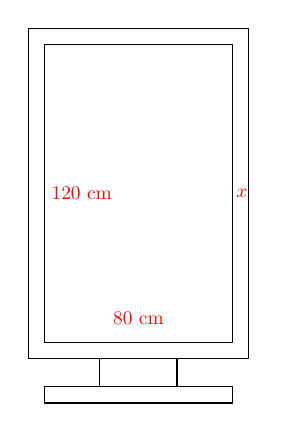
\begin{tikzpicture}[line join=round, line cap=round,scale=0.7,transform shape]
			\def\xmin{-3} \def\xmax{3}
			\def\ymin{-4} \def\ymax{3.5} 
			\draw[fill=white] (-2,-3) rectangle (2,3);
			\draw[fill=white] (-1.7,-3.8) rectangle (1.7,-3.5);
			\draw (-1.7,-2.7) rectangle (1.7,2.7);
			\draw (-.7,-3)--(-.7,-3.5) (.7,-3)--(.7,-3.5);
			\node[red] at (0,-2.5) [above]{$80$ cm};
			\node[red] at (-1.7,0) [right]{$120$ cm};
			\node[red] at (1.65,0) [right]{$x$};
	\end{tikzpicture}}
\loigiai{
	Diện tích của viền khung là $S=120\cdot 80-(120-2x)\cdot(80-2x)$, \quad $0<x<40$.\\
	Ta có
	\allowdisplaybreaks
	$\begin{aligned}[t]
		&\quad 120\cdot 80-(120-2x)\cdot(80-2x)\le 1664 \Leftrightarrow x^2-100x+416\ge 0\\
		&\Leftrightarrow \hoac{&x\le 50-2\sqrt{521} \quad \text{(thỏa mãn)}\\&x\ge 50+2\sqrt{521} \quad \text{(loại)}.}
	\end{aligned}$\\
	Vậy độ rộng của viền khung để gắn đèn led trong khoảng $(0;50-2\sqrt{521}]$.
	}
\end{bt}

\begin{bt}%[0H9Y4-1]%[Dự án đề kiểm tra HKII NH22-23-Don Lee]%[THPT CU CHI]
	Trong mặt phẳng $Oxy$, viết phương trình chính tắc của elip $4x^2+25y^2=1$ và tìm tọa độ tiêu điểm của elip đã cho.
	\loigiai{
		Ta có $4x^2+25y^2=1 \Leftrightarrow \dfrac{x^2}{\dfrac{1}{4}}+\dfrac{y^2}{\dfrac{1}{25}}=1$.\\
		Phương trình chính tắc của elip là $\dfrac{x^2}{\dfrac{1}{4}}+\dfrac{y^2}{\dfrac{1}{25}}=1$.\\
		Có $a=\dfrac{1}{2}$, $b=\dfrac{1}{5}$ suy ra $c=\dfrac{\sqrt{21}}{10}$ và tiêu điểm của elip là $F_{1}\left(-\dfrac{\sqrt{21}}{10}; 0\right)$, $F_{2}\left(\dfrac{\sqrt{21}}{10}; 0\right)$.
	}
\end{bt}

\begin{bt}%[0H9B2-2]%[0H9B3-2]%[Dự án đề kiểm tra HKII NH22-23-Don Lee]%[THPT CU CHI]
	Trong mặt phẳng $Oxy$, cho $A(3;-1)$, $B(2;5)$ và đường thẳng $\Delta\colon \heva{&x=1-2t\\&y=2t.}$
	\begin{enumerate}[a)]
		\item Viết phương trình tham số của đường thẳng đi qua hai điểm $A$, $B$.
		\item Tính chu vi tam giác $OAB$. ($O$ là gốc tọa độ)
		\item Viết phương trình đường tròn tâm $A$ và tiếp xúc $\Delta$.
	\end{enumerate}
	\loigiai{
		\begin{enumerate}[a)]
			\item Ta có $\overrightarrow{AB}=(-1;6)$ là một véc-tơ chỉ phương của đường thẳng $AB$.\\
				Phương trình tham số của $AB\colon \heva{&x=3-t\\&y=-1+6t.}$
			\item Ta có $OA=\sqrt{10}$, $OB=\sqrt{29}$, $AB=\sqrt{37}$.\\
			Suy ra $C_{OAB}=OA+OB+AB=\sqrt{10}+\sqrt{29}+\sqrt{37}$.
			\item Phương trình tổng quát của của $\Delta\colon x+y-1=0$.\\
				Gọi $R$ là bán kính của đường tròn, suy ra $R=\mathrm{d}(A,\Delta)=\dfrac{|1|}{\sqrt{2}}$.\\
				Vậy phương trình của đường tròn $(C)\colon (x-3)^2+(y+1)^2=\dfrac{1}{2}$.
		\end{enumerate}
	}
\end{bt}

\begin{bt}%[0H9B4-8]%[0H9Y4-0]%[Dự án đề kiểm tra HKII NH22-23-Don Lee]%[THPT CU CHI]
	\immini
	{Một chóa đèn pin có mặt cắt ngang có hình parabol có kích thước như hình vẽ.
	\begin{enumerate}[a)]
		\item Chọn hệ trục tọa độ $Oxy$ sao cho gốc $O$ là đỉnh của parabol và trục $Ox$ đi qua tiêu điểm. Viết phương trình chính tắc của parabol trong hệ đã chọn.
		\item Để đèn pin chiếu được xa phải đặt bóng đèn cách đỉnh của chóa đèn bao nhiêu xentimet?
	\end{enumerate}}
	{\definecolor{brightpink}{rgb}{1.0, 0.0, 0.5}
		\definecolor{ao(english)}{rgb}{0.0, 0.5, 0.0}
		\definecolor{cerulean}{rgb}{0.0, 0.48, 0.65}
		\definecolor{carnelian}{rgb}{0.7, 0.11, 0.11}
		\begin{tikzpicture}[line join = round, line cap = round,>=latex,font=\footnotesize,scale=0.6]
			\def\p{3.5}
			\def\xA{2.5}
			%	\pgfmathsetmacro{\yM}{-sqrt(2*(\p)*(\xM))}
			\coordinate (F) at (\p/2,0);
			%	\coordinate (M) at (\xM,\yM);
			\def\xmin{-1} \def\xmax{5}
			\def\ymin{-5} \def\ymax{5} 
			%	\draw[color=gray!50,dashed] (\xmin,\ymin) grid (\xmax,\ymax); 
			%	\draw[->] (\xmin,0)--(\xmax,0) node [below]{$x$};
			%	\draw[->] (0,\ymin)--(0,\ymax) node [left]{$y$};
			\node at (0,0) [left]{$24$ cm};
			\clip (\xmin+0.1,\ymin+0.1) rectangle (\xmax-0.1,\ymax-0.1);
			\draw[cerulean,line width=1,smooth,samples=100] plot[domain=0:\xA] (\x,{(2*(\p)*(\x))^(0.5)});
			\draw[cerulean,line width=1,smooth,samples=100] plot[domain=0:\xA] (\x,{-(2*(\p)*(\x))^(0.5)});
			\path
			($({1/(2*(\p)},1)$)coordinate(M)
			($({2/(\p)},2)$)coordinate(N)
			($({1/(2*(\p)},-1)$)coordinate(M')
			($({2/(\p)},-2)$)coordinate(N')
			($(\xA,{(2*(\p)*(\xA))^(0.5)})$)coordinate(A)
			($(\xA,{-(2*(\p)*(\xA))^(0.5)})$)coordinate(B)
			;
			
			\draw[cerulean,<->] (A)--(B) (0,{-(2*(\p)*(\xA))^(0.5)})--(0,{(2*(\p)*(\xA))^(0.5)});
			\draw[cerulean,<->] (0,{-(2*(\p)*(\xA))^(0.5)})--(B);
			%	\draw[brightpink,line width=1] (N)--(F)--(M) (N')--(F)--(M');
			\draw[dashed,brightpink,line width=1,->] (F)--(M);
			\draw[dashed,brightpink,line width=1,->] (F)--(N);
			\draw[dashed,brightpink,line width=1,->] (F)--(M');
			\draw[dashed,brightpink,line width=1,->] (F)--(N');
			\draw[dashed,ao(english),line width=1,->] (N)--(4,2);
			\draw[dashed,ao(english),line width=1,->] (M)--(4,1);
			\draw[dashed,ao(english),line width=1,->] (N')--(4,-2);
			\draw[dashed,ao(english),line width=1,->] (M')--(4,-1);
			\node at (1.2,-4.2) [below]{$4$ cm};
			\node at (F) [above right]{$F$};
			\fill[carnelian] (A) circle (2pt);
			\fill[carnelian] (B) circle (2pt);
	\end{tikzpicture}}
	\loigiai{
		\begin{enumerate}[a)]
			\item Gọi $(P)\colon y^2=2px \quad (p>0).$\\
				Ta có $(P)$ đi qua điểm $A(4;12)$ suy ra $12^2=2p\cdot4 \Leftrightarrow p=18$.\\
				Phương trình chính tắc của $(P)\colon y^2=36x$.
			\item Để đèn pin chiếu được xa phải đặt bóng đèn ở tiêu điểm của parabol và cách đỉnh của chóa đèn $\dfrac{p}{2}=9$ cm.
		\end{enumerate}
	}
\end{bt}